\chapter{saMKAyxreVKeyalilx baruva vividhariVtiya saMKeyxgaLu}

\begin{figure}[!h]
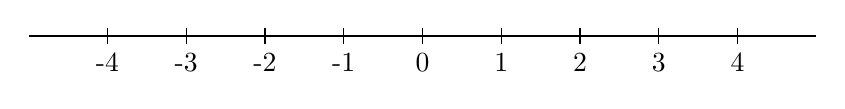
\begin{tikzpicture}
\rm \draw[thick] (-5,0)-- (5,0);
\rm \foreach \x in {-4,...,4}
\rm \draw (\x, 0.1)--(\x, -0.1) node[below]{\x};
\end{tikzpicture}
\end{figure}
idoMdu pUNARMkagaLanunx oLagoMDiruva oMdu reVKe. idanunx saMKAyxreVKe enunxtetxVve.

$0$ yiMda balagaDege iruva $1,2,3,4\ldots$ ivanunx \textbf{dhanapUNARMkagaLu} enunxtetxVve.

$0$ yiMda eDagaDege iruva $-1, -2, -3, \ldots$ ivanunx \textbf{QuNapUNARMkagaLu} enunxtetxVve.

$0$ mAtarx dhanapUNARMkavU alalx, QuNapUNARMkavU \textbf{alalx}.

$0, 1, 2, 3, 4\ldots$ ivu \textbf{pUNaRsaMKeyxgaLu}.

$1, 2, 3, 4\ldots$ ivu \textbf{sAvxBAvika} athavA \textbf{neYsagiRka saMKeyxgaLu}.

dhanapUNARMkagaLalilx $2, 4, 6, 8\ldots$ \textbf{samasaMKeyxgaLu}. aMdare {\rm 2} riMda nisheshxVSavAgi BAgavAguva saMKeyxgaLu.

dhanapUNARMkagaLalilx $1, 3, 5, 7\ldots$ \textbf{besasaMKeyxgaLu}. aMdare {\rm 2} riMda nisheshxVSavAgi BAgavAgada saMKeyxgaLu.

$4, 6, 8, 9, 12, 14, 15, 16, 18\ldots$ muMtAda saMKeyxgaLu \textbf{BAjayxsaMKeyxgaLu} ivugaLige eraDakikxMta hecucx apavataRnagaLirutatxve.

yAvudeV saMKeyxyanunx adeV saMKeyxyiMda mAtarx BAgisalu sAdhayxvAguva saMKeyxgaLu aviBAjayx saMKeyxgaLu athavA eraDeV apavataRnaviruva saMKeyxgaLige \textbf{aviBAjayx saMKeyxgaLeMdu hesaru.}

\textbf{udA}: $2, 3, 5, 7, 11, 13, 17, 19 \ldots$ {\rm 1} aviBAjayx saMKeyxyalalx {\rm 2, 3} avaLi aviBAjayxsaMKeyxgaLu {\rm 3, 5}, {\rm 11, 13} ko perxYmfsx.

$1, 4, 9, 16, 25\ldots$ muMtAda saMKeyxgaLu \textbf{vagaRsaMKeyxgaLu} aMdare oMdeV riVtiya eraDu apavataRnagaLanunx hoMdiruva saMKeyxgaLu.

$1, 8, 27, 64, 125\ldots$ muMtAda saMKeyxgaLu \textbf{Gana saMKeyxgaLu}. aMdare oMdeV riVtiya mUru apavataRnagaLanunx hoMdiruva saMKeyxgaLu.

yAvudeV sAvxBAvika saMKeyxyu tananxnunx horatupaDisi uLida apavataRgaLa motatxkekx samanAdare adu \textbf{paripUNaRsaMKeyx}.
\begin{align*}
\text{udAharaNege:}\quad  6 &= 1+2+3\\
28 &= 1+2+4+7+14\\
496 &= 1+2+4+8+16+31+62+124+248
\end{align*} 
$6,28,496\ldots$ \textbf{paripUNaRsaMKeyxgaLu}

{\rm P} matutx {\rm Q} pUNARMkagaLAdare $p/q$ rUpada saMKeyxgaLu $(q\neq 0)$ \textbf{BAgalabadhx saMKeyxgaLu}.

\textbf{udA:} {\rm 3/2, 7/4}.

${\sqrt 2}, {\sqrt 3}\ldots$ muMtAda saMKeyxgaLanunx eraDu pUNARMkagaLiMdAda BinanxrAshiya rUpadalilx bareyalu sAdhayxvilalx. ivu \textbf{aBAgalabadhxsaMKeyxgaLu}.

ivelalxvU saMKeyxgaLalilx oMdu vidhavAda neYja saMKeyxgaLu. matotxMdu riVtiyeV kalapxnA  saMKeyxgaLu. $\sqrt-1$ oMdu kalapxnAsaMKeyx {\rm Imaginary Number}. neYjasaMKeyx matutx kalapxnA saMKeyxgaLu oTuTxgUDi saMkiVNaR athavA misharx saMKeyxgaLAgutatxve. 
